% Question labels retain the original paper numbering, even where questions were omitted.
\begin{enumerate}[label=\theenumi,leftmargin=4mm,itemsep=9pt]
\setcounter{enumi}{0}\item If the quadratic equation $px^2-2\sqrt5\,px+15=0$ has two equal roots, find $p$.
\solution The equation is genuinely quadratic only when \(p\ne0\). A repeated
root is a double root in \(x\), so the discriminant condition is
\[
\Delta_x(p)=(-2\sqrt5p)^2-4p(15)=20p(p-3)=0.
\]
The nonlinear parameter equation has candidates \(p=0,3\). The value
\(p=0\) destroys the quadratic and leaves \(15=0\), so it is
inadmissible. Hence \(p=3\), and
\[
f(x;3)=3x^2-6\sqrt5x+15=3(x-\sqrt5)^2,\qquad x_*=\sqrt5.
\]
This verifies the multiplicity constraint:
\(f(x_*;3)=f_x(x_*;3)=0\), while \(f_{xx}(x_*;3)=6\ne0\).

For \(g(p)=20p(p-3)\), Newton--Raphson gives
\[
p_{k+1}=p_k-\frac{20p_k(p_k-3)}{40p_k-60}
=p_k-\frac{p_k(p_k-3)}{2p_k-3}.
\]
Both parameter roots are simple (\(g'(0)=-60,\ g'(3)=60\)), so
Newton iteration is locally quadratic near either root, except for
the singular initial value \(p_0=3/2\). The root \(p=0\) is rejected
by the original quadratic-model constraint. In contrast, Newton
iteration applied to the double root in \(x\) at \(p=3\) becomes
\[
x_{k+1}=x_k-\frac{3(x_k-\sqrt5)^2}{6(x_k-\sqrt5)}
=\frac{x_k+\sqrt5}{2}.
\]
Its error is halved on every step, showing the linear convergence
associated with a root of multiplicity two.
\begin{figure}[H]\centering
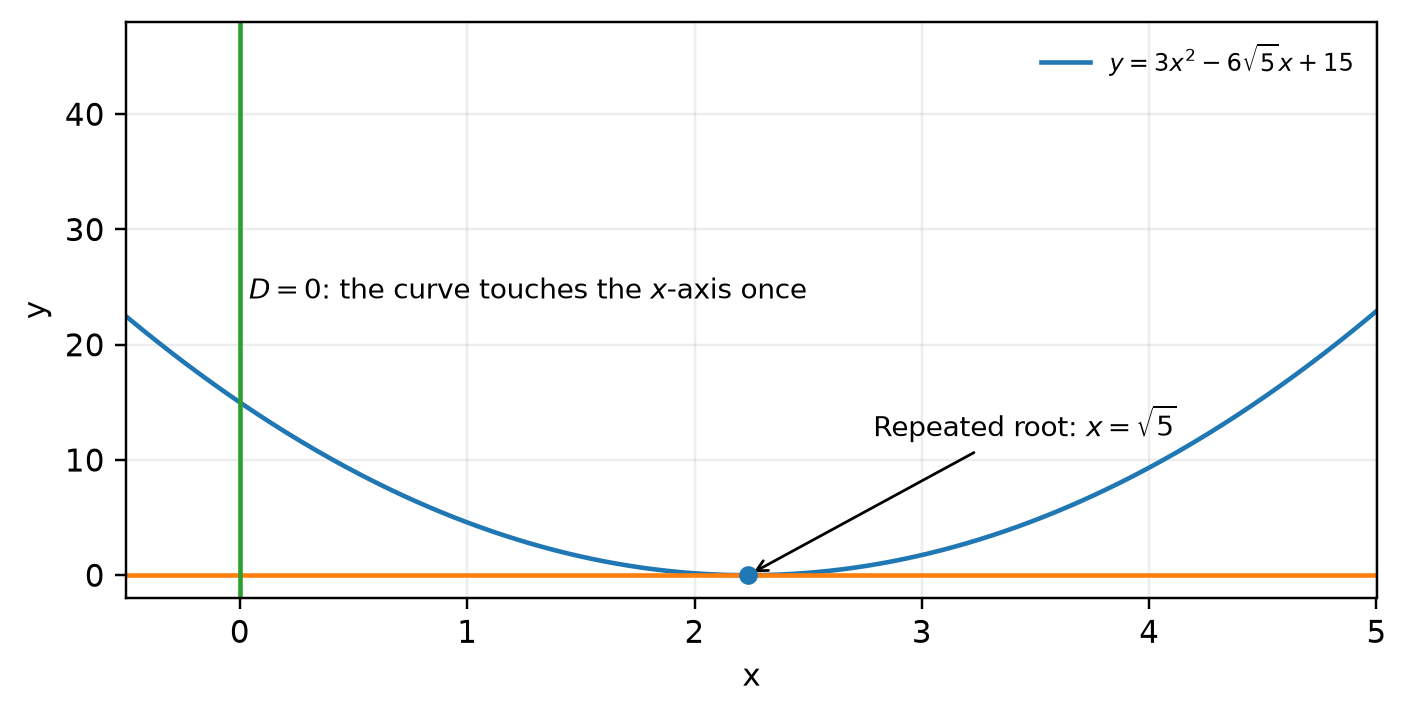
\includegraphics[width=0.92\linewidth]{../CBSE-2015-Class10-Updated-corrected_V3/figs/Q01_Quadratic.png}
\caption{At \(p=3\), the quadratic has a double root at \(x=\sqrt5\).}
\label{fig:q1-quadratic}
\end{figure}
\par\smallskip
\noindent\textbf{Code reference -}
\par\noindent\fbox{\parbox{\dimexpr\linewidth-2\fboxsep-2\fboxrule\relax}{\centering
\texttt{../CBSE-2015-Class10-Updated-corrected_V3/codes/Q01.py}}}

\setcounter{enumi}{1}\item A tower $AB$ is $20\,\mathrm m$ high and its shadow $BC$ is $20\sqrt3\,\mathrm m$ long. Find the Sun's altitude.
\begin{figure}[H]\centering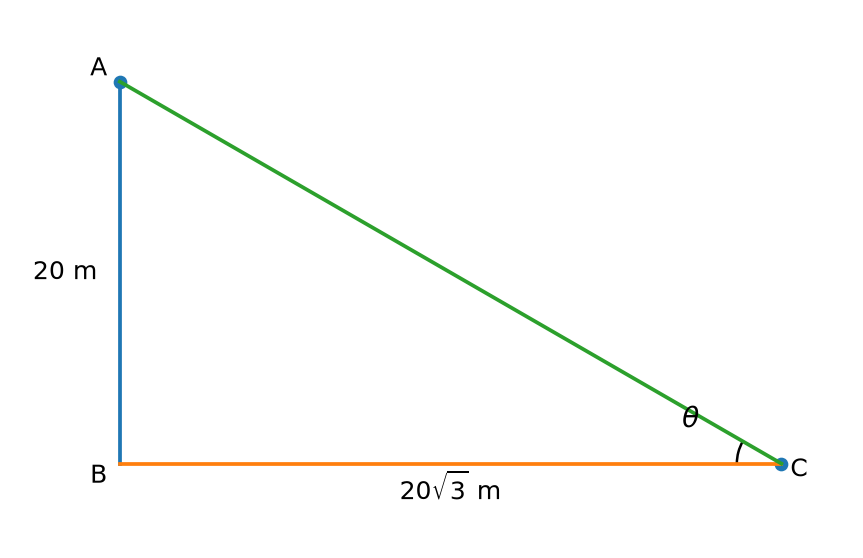
\includegraphics[width=0.78\linewidth]{../CBSE-2015-Class10-Updated-corrected_V3/figs/Tower.png}\caption{Tower and its shadow.}\label{fig:tower}\end{figure}
\solution Let the angle of elevation be $\theta$. From the right triangle,
\begin{equation*}
\tan\theta=\frac{AB}{BC}=\frac{20}{20\sqrt3}=\frac1{\sqrt3}\qquad\eqref{eq:trig-ratios}.
\end{equation*}
Thus $\theta=30^\circ$.



The tower-and-shadow diagram is generated by this script:
\par\smallskip
\noindent\textbf{Code reference -}
\par\noindent\fbox{\parbox{\dimexpr\linewidth-2\fboxsep-2\fboxrule\relax}{\centering\texttt{../CBSE-2015-Class10-Updated-corrected_V3/codes/Q02.py}}}
\par\smallskip
\newpage
\setcounter{enumi}{2}\item Two different dice are tossed together. Find the probability that the product of their top numbers is $6$.
\solution Let \(X,Y\) be the top numbers on the distinguishable dice.
They are independent discrete uniform random variables on
\(\{1,\ldots,6\}\), so \(P(X=i,Y=j)=1/36\). Define \(Z=XY\).
Its probability mass function is the push-forward of the joint law
under the map \((i,j)\mapsto ij\):
\[
p_Z(m)=P(Z=m)=
\sum_{i=1}^{6}\sum_{j=1}^{6}\frac1{36}\mathbf1_{\{ij=m\}}.
\]
The four ordered factor pairs producing \(m=6\) are
\((1,6),(2,3),(3,2),(6,1)\), so
\[
P(Z=6)=p_Z(6)=\frac4{36}=\boxed{\frac19}.
\]
The probability-generating function is
\[
G_Z(s)=E[s^Z]=\frac1{36}\sum_{i=1}^{6}\sum_{j=1}^{6}s^{ij};
\]
the coefficient of \(s^6\) is \(1/9\). Probability is conserved:
\[
\sum_m p_Z(m)=\frac1{36}
\sum_{i=1}^{6}\sum_{j=1}^{6}1=1.
\]
\begin{figure}[H]\centering
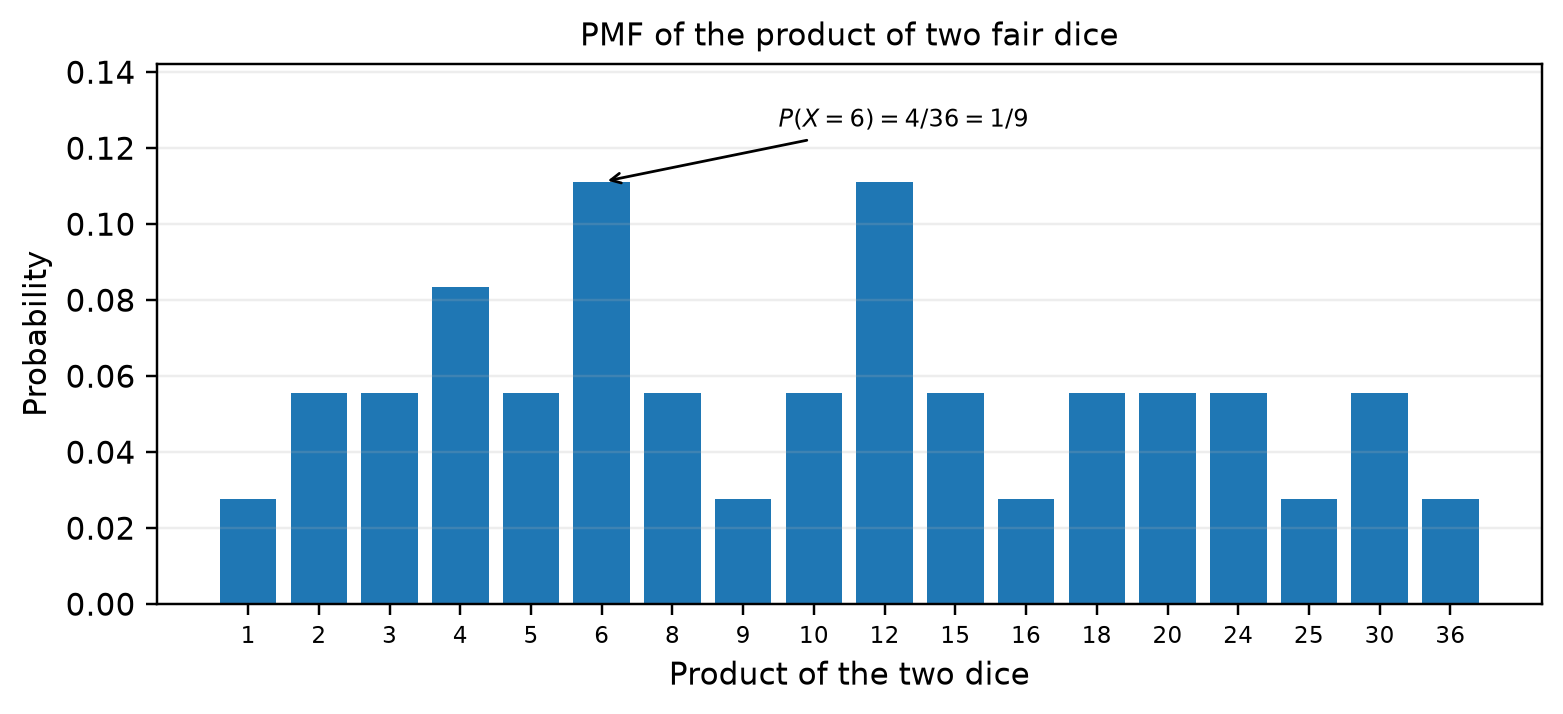
\includegraphics[width=0.98\linewidth]{../CBSE-2015-Class10-Updated-corrected_V3/figs/Q03_ProductPMF.png}
\caption{Push-forward probability mass function of the product of two fair dice.}
\label{fig:q3-pmf}
\end{figure}
\par\smallskip
\noindent\textbf{Code reference -}
\par\noindent\fbox{\parbox{\dimexpr\linewidth-2\fboxsep-2\fboxrule\relax}{\centering
\texttt{../CBSE-2015-Class10-Updated-corrected_V3/codes/Q03.py}}}

\newpage
\setcounter{enumi}{3}\item $PQ$ is a chord of a circle with centre $O$, and $PT$ is a tangent. If $\angle QPT=60^\circ$, find $\angle PRQ$.
\begin{figure}[H]\centering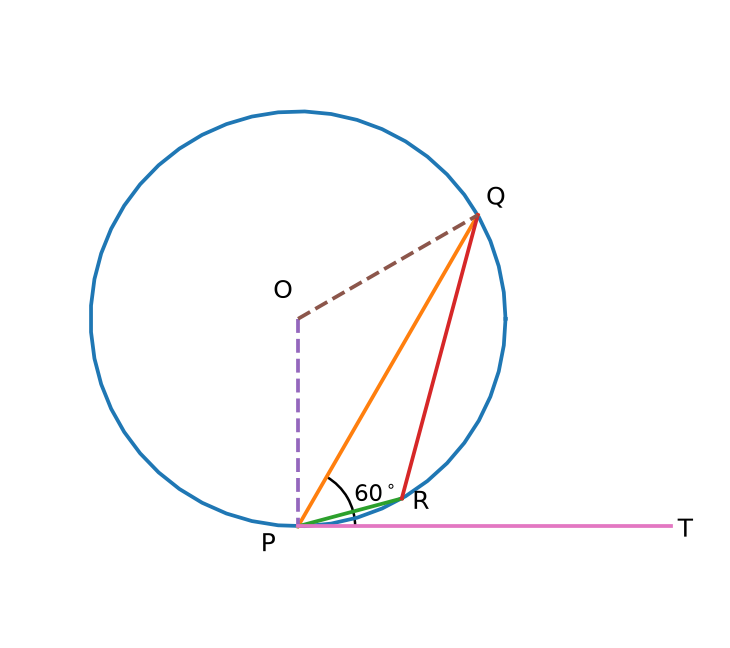
\includegraphics[width=0.72\linewidth]{../CBSE-2015-Class10-Updated-corrected_V3/figs/TangentChord.png}\caption{Chord--tangent configuration.}\label{fig:tangent-chord}\end{figure}
\solution Since $OP\perp PT$, we have $\angle OPQ=30^\circ$. As $OP=OQ$, triangle $OPQ$ is isosceles, so $\angle OQP=30^\circ$ and $\angle POQ=120^\circ$. With $R$ on the minor arc $PQ$, the intercepted major arc measures $240^\circ$. An angle at the circumference is half its intercepted arc, hence $\angle PRQ=120^\circ$. The tangent--chord theorem gives the alternate-segment angle as $60^\circ$, consistent with the supplementary angle here \qquad\eqref{eq:tangent-chord}.


The circle-and-tangent diagram is generated by this script:
\par\smallskip
\noindent\textbf{Code reference -}
\par\noindent\fbox{\parbox{\dimexpr\linewidth-2\fboxsep-2\fboxrule\relax}{\centering\texttt{../CBSE-2015-Class10-Updated-corrected_V3/codes/Q04.py}}}
\par\smallskip
\newpage
\setcounter{enumi}{5}\item A triangle circumscribes a circle of radius $3\,\mathrm{cm}$. The base portions are $BD=6\,\mathrm{cm}$ and $DC=9\,\mathrm{cm}$. If the triangle's area is $54\,\mathrm{cm}^2$, find $AB$ and $AC$.
\begin{figure}[H]\centering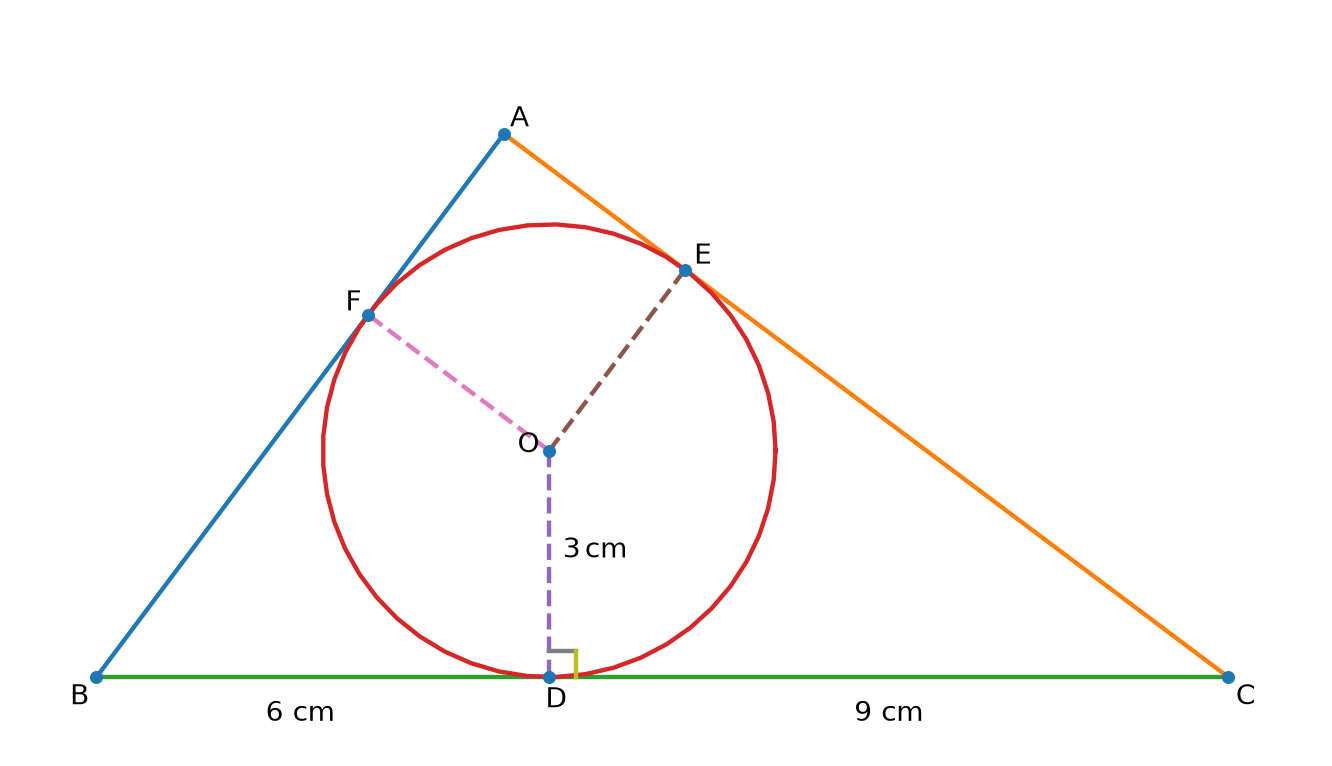
\includegraphics[width=0.78\linewidth]{../CBSE-2015-Class10-Updated-corrected_V3/figs/IncircleTriangle.png}\caption{Triangle with an incircle.}\label{fig:incircle}\end{figure}
\solution The semiperimeter is
\begin{equation*}
s=\frac{[ABC]}r=\frac{54}{3}=18\,\mathrm{cm}\qquad\eqref{eq:triangle-inradius}.
\end{equation*}
Tangents from a common external point have equal lengths. Let the tangent length from $A$ be $x$. Then $AB=x+6$, $AC=x+9$, and $BC=15$ \qquad\eqref{eq:equal-tangents}. Consequently,
\begin{equation*}
s=\frac{(x+6)+(x+9)+15}{2}=x+15=18,
\end{equation*}
so $x=3$. Therefore $AB=9\,\mathrm{cm},\quad AC=12\,\mathrm{cm}$.



The incircle diagram is generated by this script:
\par\smallskip
\noindent\textbf{Code reference -}
\par\noindent\fbox{\parbox{\dimexpr\linewidth-2\fboxsep-2\fboxrule\relax}{\centering\texttt{../CBSE-2015-Class10-Updated-corrected_V3/codes/Q06.py}}}
\par\smallskip
\newpage
\setcounter{enumi}{7}\item In an arithmetic progression, $S_5+S_7=167$ and $S_{10}=235$. Find the AP.
\solution Let \(x=(a,d)^T\). The conditions on the progression give
\[
Ax=b,\qquad A=\begin{pmatrix}12&31\\10&45\end{pmatrix},
\quad b=\begin{pmatrix}167\\235\end{pmatrix}.
\]
For \(A=D+L+U\), with \(D=\operatorname{diag}(12,45)\), the
Jacobi iteration is
\[
x^{(k+1)}=D^{-1}\bigl(b-(L+U)x^{(k)}\bigr)
=B_Jx^{(k)}+D^{-1}b,
\quad B_J=\begin{pmatrix}0&-31/12\\-2/9&0\end{pmatrix}.
\]
The characteristic equation is
\[
\lambda^2-\frac{31}{54}=0,\quad
\lambda_\pm=\pm\sqrt{\frac{31}{54}},\quad
\rho(B_J)=\sqrt{\frac{31}{54}}\approx0.757677<1.
\]
Thus Jacobi converges for every initial guess. Starting at
\(x^{(0)}=(0,0)^T\), the iterates converge to \(x^*=(1,5)^T\).
The residual norm \(\|Ax^{(k)}-b\|_2\) is approximately
\(1.121\), \(4.36\times10^{-3}\), \(1.69\times10^{-5}\), and
\(6.6\times10^{-8}\) after 20, 40, 60, and 80 iterations,
respectively. A suitable stopping rule requires both a small relative
iterate change and residual at most \(10^{-6}\). Therefore
\[
\boxed{a=1,\ d=5},\qquad 1,6,11,16,\ldots
\]
The negative eigenvalue explains the alternating component of
convergence; the verification script implements Jacobi directly.
\par\smallskip
\noindent\textbf{Code reference -}
\par\noindent\fbox{\parbox{\dimexpr\linewidth-2\fboxsep-2\fboxrule\relax}{\centering
\texttt{../CBSE-2015-Class10-Updated-corrected_V3/codes/Q08.py}}}

\setcounter{enumi}{8}\item $A(4,7)$, $B(p,3)$ and $C(7,3)$ form a right triangle, right-angled at $B$. Find $p$.
\solution The two side vectors meeting at $B$ are
\begin{equation*}
\overrightarrow{BA}=\myvec{4-p\\4},\qquad \overrightarrow{BC}=\myvec{7-p\\0}.
\end{equation*}
Since the sides are perpendicular, their inner product is zero:
\begin{equation*}
\langle\overrightarrow{BA},\overrightarrow{BC}\rangle=(4-p)(7-p)=0\qquad\eqref{eq:right-angle-dot}.
\end{equation*}
Thus $p=4$ or $p=7$. The second value makes $B=C$, so it does not form a triangle. Hence $p=4$.




\setcounter{enumi}{9}\item If $A(x,y)$, $B(-5,7)$ and $C(-4,5)$ are collinear, find the relation between $x$ and $y$.
\solution Place the three points in the homogeneous-coordinate matrix
\[
M=\begin{pmatrix}x&y&1\\-5&7&1\\-4&5&1\end{pmatrix}.
\]
Collinearity is equivalent to linear dependence of the three rows,
or \(\operatorname{rank}(M)\le2\). Since the last two points are
distinct, the rank is at least two; hence the condition is
\(\det M=0\). Subtracting the second row from the first and third gives
\[
\det M=
\begin{vmatrix}x+5&y-7\\1&-2\end{vmatrix}
=-2(x+5)-(y-7).
\]
Thus the required relation is
\[
\boxed{2x+y+3=0}.
]

\newpage
\setcounter{enumi}{10}\item The 14th term of an AP is twice its 8th term. If the 6th term is $-8$, find the sum of its first 20 terms.
\solution Represent the AP as the one-sided sequence
\(x[n]=a+(n-1)d\), \(n\ge1\), with \(x[0]=0\). Its unilateral
\(Z\)-transform is
\[
X(z)=\sum_{n=1}^{\infty}(a+(n-1)d)z^{-n}
=\frac{a}{z-1}+\frac{d}{(z-1)^2},\qquad |z|>1.
\]
The term constraints give \(a+13d=2(a+7d)\), so \(a+d=0\);
also \(a+5d=-8\). Thus \(a=2\) and \(d=-2\).
For the cumulative sequence \(s[n]=\sum_{k=1}^{n}x[k]\),
\[
S(z)=\frac{X(z)}{1-z^{-1}},
\]
the unilateral accumulation relation. Inverting it gives
\(s[n]=na+\frac{n(n-1)}2d\), so
\[
S_{20}=s[20]=20(2)+\frac{20\cdot19}{2}(-2)
=\boxed{-340}.
]

\setcounter{enumi}{12}\item An aeroplane is observed at an elevation of $60^\circ$ from point $A$. After 15 seconds, the elevation becomes $30^\circ$. If its altitude remains $1500\sqrt3\,\mathrm m$, find its speed in km/h.
\begin{figure}[H]\centering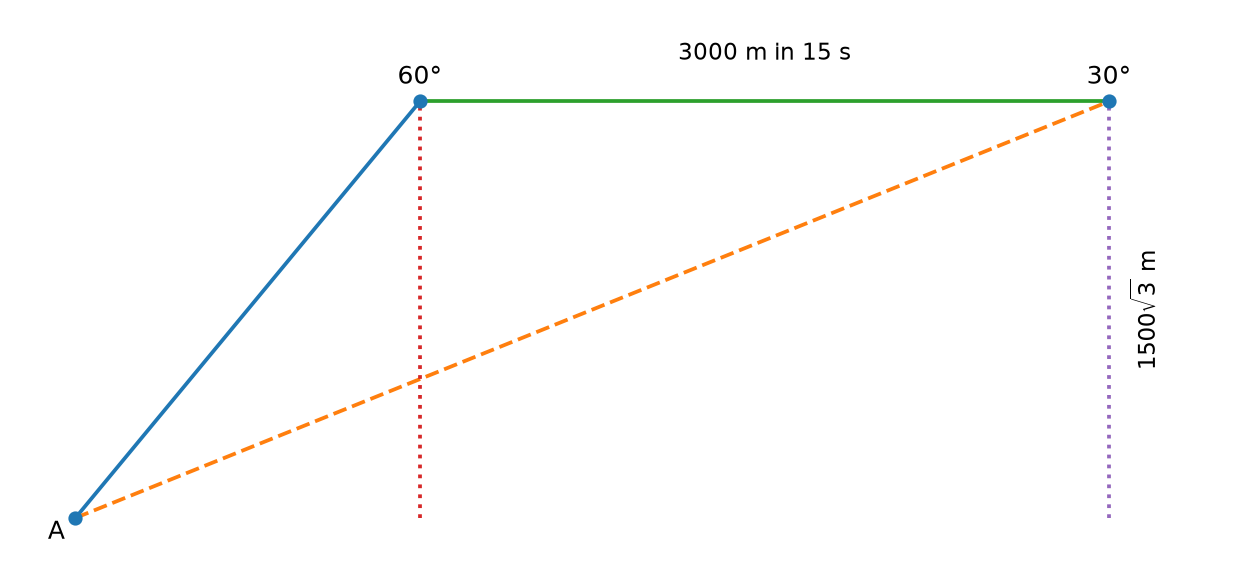
\includegraphics[width=0.86\linewidth]{../CBSE-2015-Class10-Updated-corrected_V3/figs/Aeroplane.png}\caption{The plane moves horizontally while staying at the same altitude.}\label{fig:aeroplane}\end{figure}
\solution Let its initial and final horizontal ranges be $x_1$ and $x_2$. Since the altitude $h$ is fixed, $x=h\cot\theta$:
\begin{align*}
x_1&=1500\sqrt3\cot60^\circ=1500\,\mathrm m,\\
x_2&=1500\sqrt3\cot30^\circ=4500\,\mathrm m\qquad\eqref{eq:horizontal-range}.
\end{align*}
The plane covers $x_2-x_1=3000\,\mathrm m$ in 15 s. Therefore,
\begin{equation*}
v=\frac{3000}{15}=200\,\mathrm{m/s}=200\times\frac{18}{5}=720\,\mathrm{km/h}\qquad\eqref{eq:speed-time}.
\end{equation*}



The speed calculation and accompanying figure are generated by this script:
\par\smallskip
\noindent\textbf{Code reference -}
\par\noindent\fbox{\parbox{\dimexpr\linewidth-2\fboxsep-2\fboxrule\relax}{\centering\texttt{../CBSE-2015-Class10-Updated-corrected_V3/codes/Q13.py}}}
\par\smallskip
\newpage
\setcounter{enumi}{13}\item $A(-2,-2)$ and $B(2,-4)$. Find the point $P$ on segment $AB$ for which $AP=\frac37 AB$.
\begin{figure}[H]\centering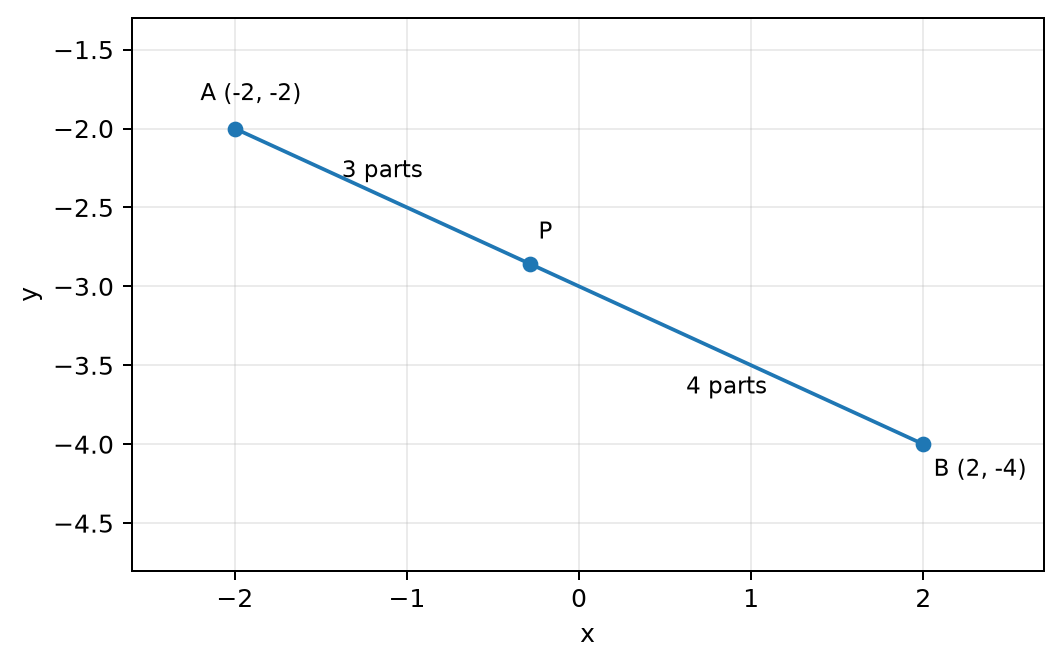
\includegraphics[width=0.82\linewidth]{../CBSE-2015-Class10-Updated-corrected_V3/figs/SectionPoint.png}\caption{The point $P$ is three-sevenths of the way from $A$ to $B$.}\label{fig:section-point}\end{figure}
\solution The section formula gives
\begin{align*}
\vec p&=\vec a+\frac37(\vec b-\vec a)\qquad\eqref{eq:vector-basics},\ \eqref{eq:section-vector}\\
&=\myvec{-2\\-2}+\frac37\myvec{4\\-2}=\myvec{-2/7\\-20/7}.
\end{align*}
Hence $P\left(-\frac27,-\frac{20}{7}\right)$.



The section-formula diagram is generated by this script:
\par\smallskip
\noindent\textbf{Code reference -}
\par\noindent\fbox{\parbox{\dimexpr\linewidth-2\fboxsep-2\fboxrule\relax}{\centering\texttt{../CBSE-2015-Class10-Updated-corrected_V3/codes/Q14.py}}}
\par\smallskip
\setcounter{enumi}{14}\item A jar contains only red, blue and orange balls. The probabilities of drawing a red and a blue ball are $\frac14$ and $\frac13$, respectively. If there are 10 orange balls, find the total number of balls.
\solution Let $N$ be the total number of balls. Write each probability separately:
\begin{align*}
P(R)&=\frac{\text{number of red balls}}{N}=\frac14,\\
P(B)&=\frac{\text{number of blue balls}}{N}=\frac13,\\
P(O)&=\frac{\text{number of orange balls}}{N}=\frac{10}{N}.
\end{align*}
Since every ball is one of these three colours, $P(R)+P(B)+P(O)=1\qquad\eqref{eq:three-events}$. Thus
\begin{equation*}
\frac14+\frac13+\frac{10}{N}=1\quad\Longrightarrow\quad\frac{10}{N}=\frac5{12}\quad\Longrightarrow\quad N=24.
\end{equation*}
So there are $24$ balls in total: 6 red, 8 blue and 10 orange.



\begin{figure}[H]\centering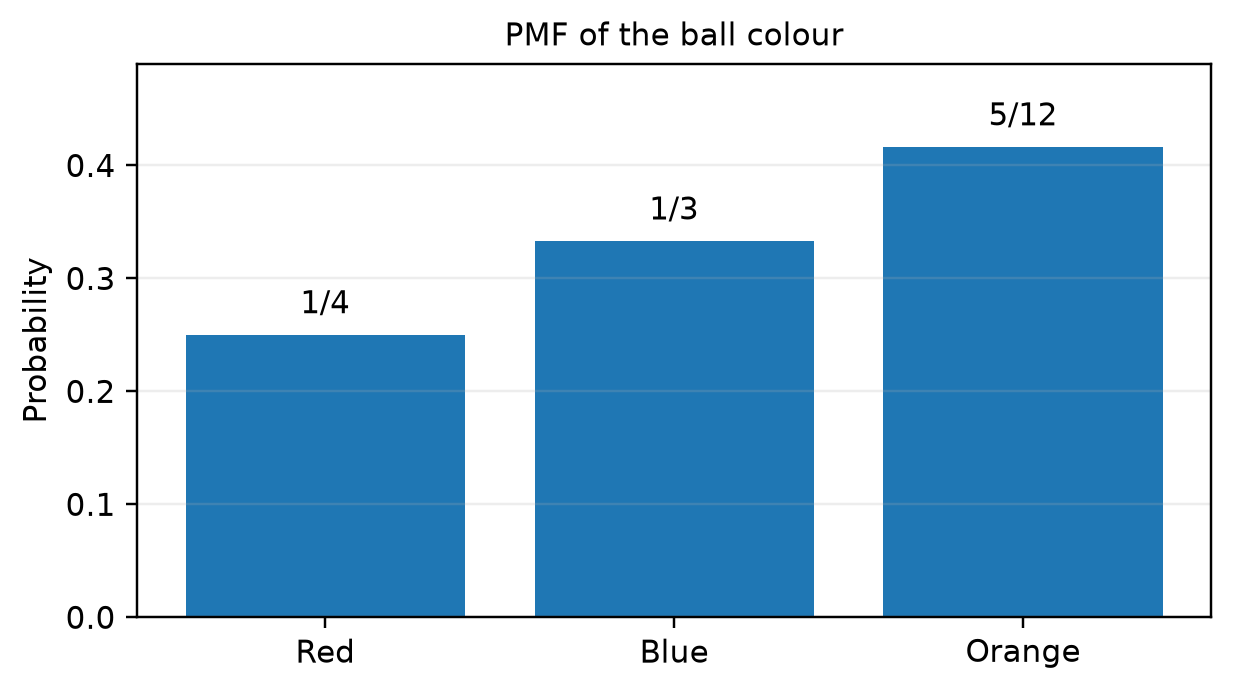
\includegraphics[width=0.9\linewidth]{../CBSE-2015-Class10-Updated-corrected_V3/figs/Q15_ColourPMF.png}\caption{Probability mass function for drawing each ball colour. The three probabilities sum to 1.}\label{fig:q15-pmf}\end{figure}
The Python code plots the theoretically derived probabilities $1/4$, $1/3$, and $5/12$ as a probability mass function:
\par\smallskip
\noindent\textbf{Code reference -}
\par\noindent\fbox{\parbox{\dimexpr\linewidth-2\fboxsep-2\fboxrule\relax}{\centering\texttt{../CBSE-2015-Class10-Updated-corrected_V3/codes/Q15.py}}}
\par\smallskip
\newpage
\setcounter{enumi}{15}\item Find the minor and major segment areas of a circle of radius $14\,\mathrm{cm}$ cut by a chord subtending $60^\circ$ at the centre. Use $\pi=\frac{22}{7}$.
\begin{figure}[H]\centering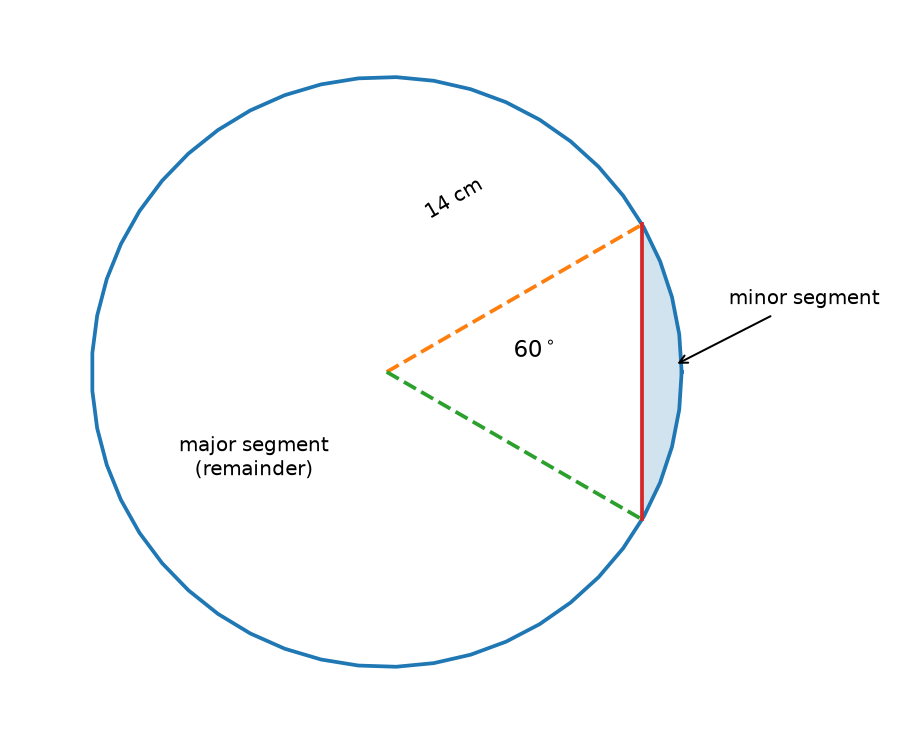
\includegraphics[width=0.86\linewidth]{../CBSE-2015-Class10-Updated-corrected_V3/figs/SegmentAreas.png}\caption{The minor segment is the small cap; the major segment is the remainder of the circle.}\label{fig:segment-areas}\end{figure}
\solution The sector angle is $60^\circ$, so
\begin{equation*}
A_{\mathrm{sector}}=\frac{60}{360}\pi(14)^2=\frac{308}{3}\,\mathrm{cm}^2\qquad\eqref{eq:sector-segment}.
\end{equation*}
The triangle between the two radii has two sides 14 cm and included angle $60^\circ$, so it is equilateral. Its area is $\frac{\sqrt3}{4}(14)^2=49\sqrt3\,\mathrm{cm}^2$. Subtracting this triangle from the sector gives
\begin{equation*}
A_{\mathrm{minor}}=\frac{308}{3}-49\sqrt3\,\mathrm{cm}^2.
\end{equation*}
The whole circle has area $\pi(14)^2=616\,\mathrm{cm}^2$. Therefore
\begin{equation*}
A_{\mathrm{major}}=616-A_{\mathrm{minor}}=\frac{1540}{3}+49\sqrt3\,\mathrm{cm}^2.
\end{equation*}



The segment diagram and area check are generated by this script:
\par\smallskip
\noindent\textbf{Code reference -}
\par\noindent\fbox{\parbox{\dimexpr\linewidth-2\fboxsep-2\fboxrule\relax}{\centering\texttt{../CBSE-2015-Class10-Updated-corrected_V3/codes/Q16.py}}}
\par\smallskip
\newpage
\setcounter{enumi}{16}\item One tent has a cylindrical lower part of diameter $4.2\,\mathrm m$ and height $4\,\mathrm m$, topped by a cone with the same diameter and height $2.8\,\mathrm m$. Canvas costs Rs. 100 per $\mathrm m^2$. Find the associations' 50\% contribution for 100 tents, and state the values shown.
\begin{figure}[H]\centering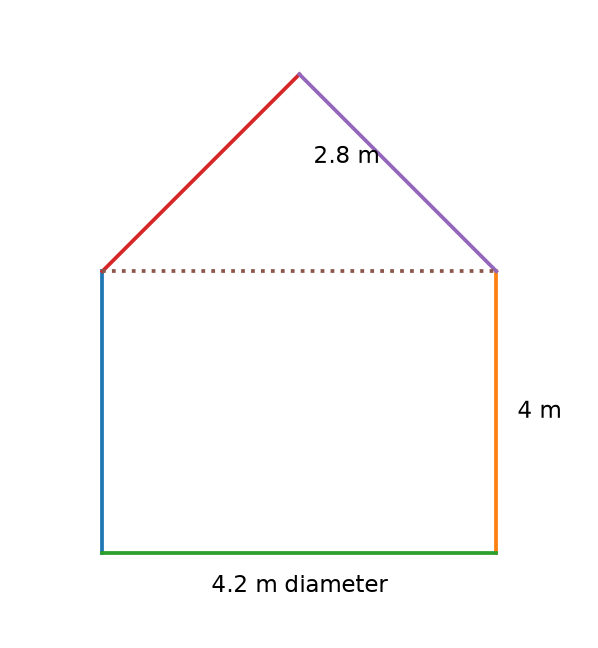
\includegraphics[width=0.72\linewidth]{../CBSE-2015-Class10-Updated-corrected_V3/figs/Tent.png}\caption{The tent consists of a cylinder and a cone and has no canvas floor.}\label{fig:tent}\end{figure}
\solution The radius is $r=2.1\,\mathrm m$. The cone's slant height is
\begin{equation*}
\ell=\sqrt{2.1^2+2.8^2}=3.5\,\mathrm m\qquad\eqref{eq:cone-formula}.
\end{equation*}
Only the curved cylinder and cone surfaces need canvas. Their combined area is
\begin{align*}
A&=2\pi rh+\pi r\ell\qquad\eqref{eq:cone-formula}\\
&=2\pi(2.1)(4)+\pi(2.1)(3.5)=75.9\,\mathrm m^2.
\end{align*}
For 100 tents, the total cost is $100\times75.9\times100=\text{Rs. }759{,}000$. Half is $\text{Rs. }379{,}500$. The plan also shows cooperation, initiative and care for people affected by floods.


The tent cross-section is generated by this script:
\par\smallskip
\noindent\textbf{Code reference -}
\par\noindent\fbox{\parbox{\dimexpr\linewidth-2\fboxsep-2\fboxrule\relax}{\centering\texttt{../CBSE-2015-Class10-Updated-corrected_V3/codes/Q17.py}}}
\par\smallskip
\setcounter{enumi}{21}\item Find the 60th term of the AP $8,10,12,\ldots$ and the sum of its last 10 terms.
\solution Here $a=8$ and $d=2$.
\begin{equation*}
t_{60}=8+59(2)=126\qquad\eqref{eq:ap}.
\end{equation*}
The 51st term is $t_{51}=8+50(2)=108$. The last ten terms run from 108 to 126, so
\begin{equation*}
S_{51\ldots60}=S_{60}-S_{50}=\frac{10}{2}(108+126)=1170\qquad\eqref{eq:ap-subsum}.
\end{equation*}



The 60th term and final-ten-term sum are checked by this script:
\par\smallskip
\noindent\textbf{Code reference -}
\par\noindent\fbox{\parbox{\dimexpr\linewidth-2\fboxsep-2\fboxrule\relax}{\centering\texttt{../CBSE-2015-Class10-Updated-corrected_V3/codes/Q22.py}}}
\par\smallskip
\setcounter{enumi}{26}\item Point $A$ is 20 m above a lake. The angle of elevation of a cloud is $30^\circ$, while the angle of depression of its reflection in the lake is $60^\circ$. Find the distance from $A$ to the cloud.
\begin{figure}[H]\centering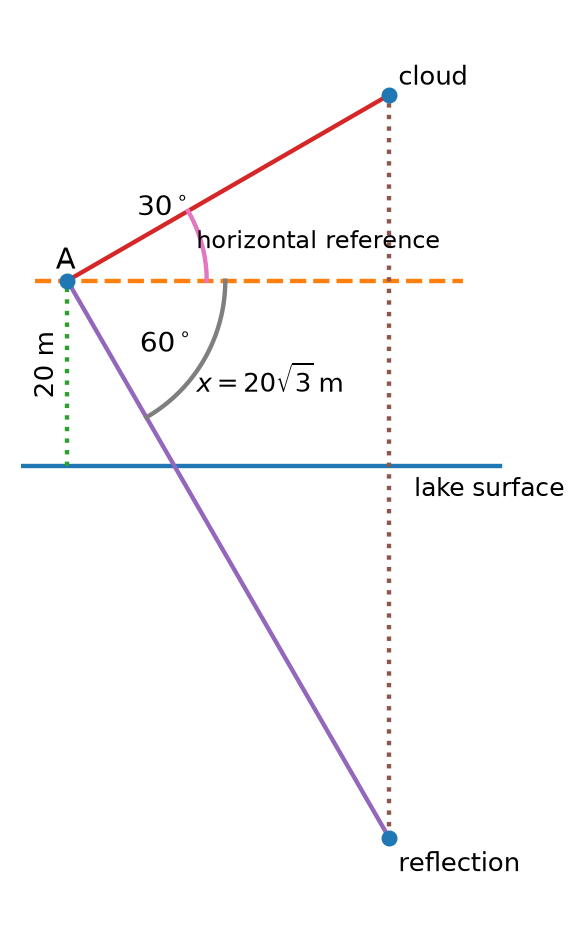
\includegraphics[height=0.42\textheight,keepaspectratio]{../CBSE-2015-Class10-Updated-corrected_V3/figs/CloudReflection.png}\caption{The reflection is as far below the lake surface as the cloud is above it.}\label{fig:cloud-reflection}\end{figure}
\solution Let $H$ be the cloud's height above the lake and let $x$ be the horizontal distance from $A$ to the vertical line through the cloud. The cloud is $H-20$ metres above $A$, while its reflection is $H+20$ metres below $A$. As shown in the figure, both the angle of elevation and the angle of depression are measured from the horizontal reference line through $A$. Using the two angles,
\begin{align*}
\frac{H-20}{x}&=\tan30^\circ=\frac1{\sqrt3},\\
\frac{H+20}{x}&=\tan60^\circ=\sqrt3.\qquad\eqref{eq:trig-ratios},\ \eqref{eq:horizontal-range}
\end{align*}
Rearranging produces a linear system in the unknowns $H$ and $x$:
\begin{equation*}
\myvec{1&-1/\sqrt3\\1&-\sqrt3}\myvec{H\\x}=\myvec{20\\-20}.
\end{equation*}
For clarity, solve this system by Gaussian elimination. Its augmented matrix is
\begin{equation*}
\left[\begin{array}{cc|c}1&-1/\sqrt3&20\\1&-\sqrt3&-20\end{array}\right]
\xrightarrow{\;R_2\leftarrow R_2-R_1\;}
\left[\begin{array}{cc|c}1&-1/\sqrt3&20\\0&-2/\sqrt3&-40\end{array}\right].
\end{equation*}
The second row gives $-2x/\sqrt3=-40$, so $x=20\sqrt3\,\mathrm m$. Substitution into the first row yields $H-20=20$, so $H=40\,\mathrm m$. Hence the vertical separation between $A$ and the cloud is $H-20=20\,\mathrm m$. By Pythagoras,
\begin{equation*}
AC=\sqrt{x^2+(H-20)^2}=\sqrt{(20\sqrt3)^2+20^2}=40\,\mathrm m.
\end{equation*}



The linear system is solved independently and the angle diagram is generated by this script:
\par\smallskip
\noindent\textbf{Code reference -}
\par\noindent\fbox{\parbox{\dimexpr\linewidth-2\fboxsep-2\fboxrule\relax}{\centering\texttt{../CBSE-2015-Class10-Updated-corrected_V3/codes/Q27.py}}}
\par\smallskip
\setcounter{enumi}{27}\item A card is drawn from a well-shuffled 52-card deck. Find the probability that it is (i) a spade or an ace, (ii) a black king, (iii) neither a jack nor a king, (iv) either a king or a queen.
\solution Use the classical probability and union rules:
\begin{enumerate}[label=(\roman*)]
\item The 13 spades and 4 aces overlap at the ace of spades. Thus $P=(13+4-1)/52=4/13\qquad\eqref{eq:prob-classical}, \eqref{eq:prob-union}$.
\item There are two black kings, so $P=2/52=1/26\qquad\eqref{eq:prob-classical}$.
\item There are four jacks and four kings. Their complement contains $52-4-4=44$ cards, so $P=44/52=11/13\qquad\eqref{eq:prob-classical}$.
\item Kings and queens are disjoint categories, each with four cards. Thus $P=(4+4)/52=2/13\qquad\eqref{eq:prob-classical}$.
\end{enumerate}

\setcounter{enumi}{28}\item Find $k$ if the triangle with vertices $(1,-1)$, $(-4,2k)$ and $(-k,-5)$ has area 24 square units.
\solution Taking differences of the coordinate vectors,
\begin{equation*}
2[ABC]=\left|\mydet{-5&2k+1\\-k-1&-4}\right|\qquad\eqref{eq:triangle-det}.
\end{equation*}
Expanding the determinant gives
\begin{equation*}
2[ABC]=|2k^2+3k+21|.
\end{equation*}
Since $2k^2+3k+21$ has positive leading coefficient and discriminant $9-168=-159<0$, it is positive for every real $k$. The specified area is 24, so the determinant's absolute value is 48 and
\begin{equation*}
2k^2+3k+21=48\quad\Longrightarrow\quad2k^2+3k-27=0.
\end{equation*}
Applying the quadratic formula, the discriminant is $3^2-4(2)(-27)=225$, hence
\begin{equation*}
k=\frac{-3\pm\sqrt{225}}4=\frac{-3\pm15}4.
\end{equation*}
Therefore both solutions are valid: $k=3\quad\text{or}\quad k=-\frac92$.



\begin{figure}[H]\centering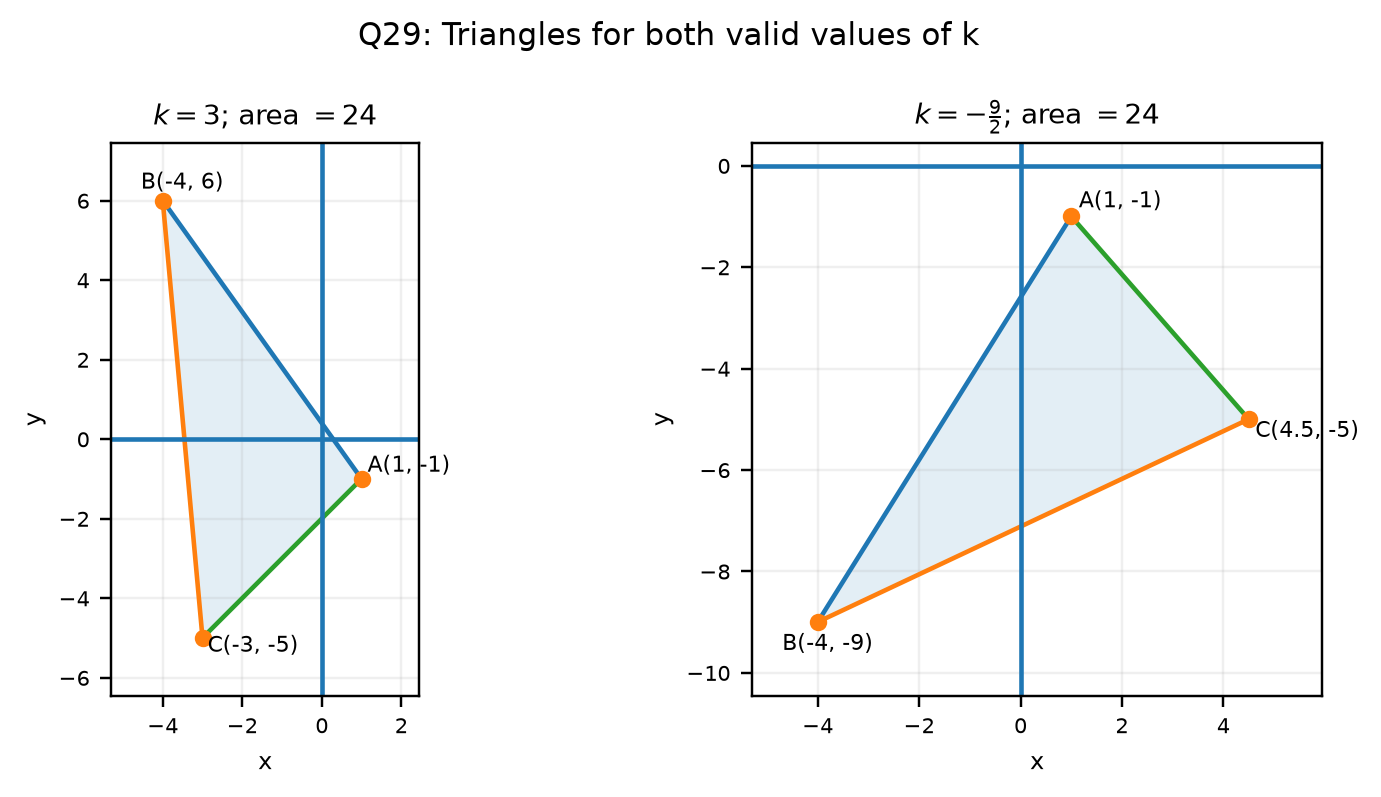
\includegraphics[width=0.99\linewidth]{../CBSE-2015-Class10-Updated-corrected_V3/figs/Q29_Triangles.png}\caption{The triangle formed by the given coordinates for each valid solution, $k=3$ and $k=-\frac92$. Both triangles have area 24 square units.}\label{fig:q29-triangles}\end{figure}
The Python code plots the triangles for the two theoretically derived values of $k$, using the coordinate area formula for the displayed areas:
\par\smallskip
\noindent\textbf{Code reference -}
\par\noindent\fbox{\parbox{\dimexpr\linewidth-2\fboxsep-2\fboxrule\relax}{\centering\texttt{../CBSE-2015-Class10-Updated-corrected_V3/codes/Q29.py}}}
\par\smallskip
\setcounter{enumi}{29}\item A square lawn has side 42 m. Two circular flower beds lie outside the vertical sides, with each circle centred at the intersection $O$ of the square's diagonals. Find the total shaded area. Use $\pi=22/7$.
\begin{figure}[H]\centering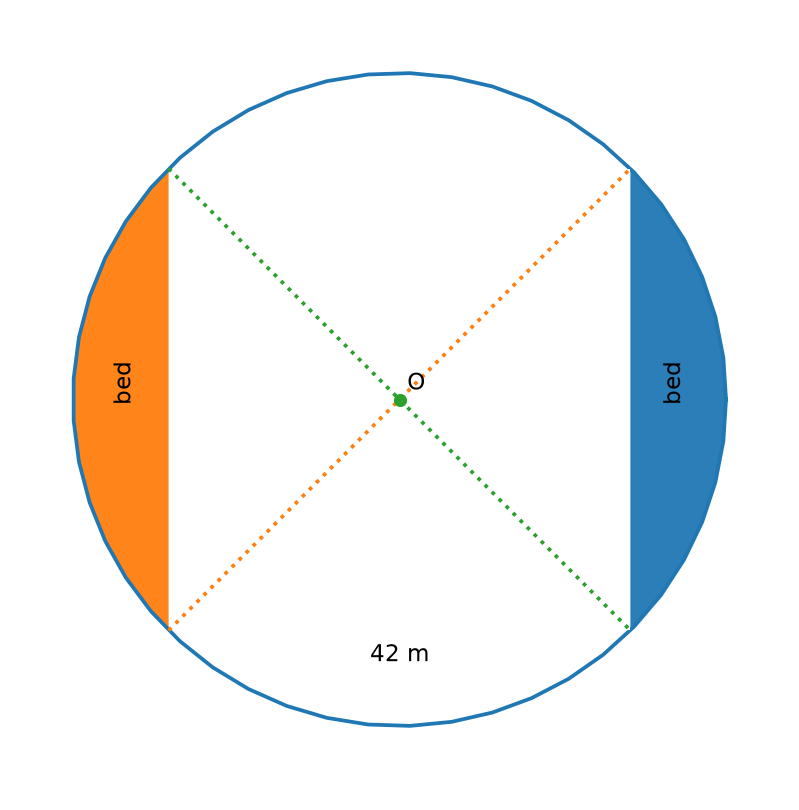
\includegraphics[width=0.84\linewidth]{../CBSE-2015-Class10-Updated-corrected_V3/figs/FlowerBeds.png}\caption{The shaded parts are the two circular segments outside the square lawn.}\label{fig:flower-beds}\end{figure}
\solution The radius from the centre to a corner is half the diagonal. Thus
\begin{equation*}
r^2=\frac{42^2+42^2}{4}=882\,\mathrm{m}^2.
\end{equation*}
Each vertical side subtends $90^\circ$ at $O$. The area of one segment is the area of a quarter-circle sector minus the right triangle with legs 21 m and 21 m:
\begin{equation*}
A_1=\frac14\pi r^2-\frac12(42/2)^2=\frac{882\pi}{4}-441.
\end{equation*}
The two beds are congruent, so
\begin{equation*}
A_{\mathrm{total}}=2A_1=441\pi-882\qquad\eqref{eq:shaded-area}.
\end{equation*}
Using $\pi=22/7$ gives $A_{\mathrm{total}}=1386-882=504\,\mathrm{m}^2$.



The flower-bed figure and shaded-area result are generated by this script:
\par\smallskip
\noindent\textbf{Code reference -}
\par\noindent\fbox{\parbox{\dimexpr\linewidth-2\fboxsep-2\fboxrule\relax}{\centering\texttt{../CBSE-2015-Class10-Updated-corrected_V3/codes/Q30.py}}}
\par\smallskip
\setcounter{enumi}{30}\item From both ends of a metal cylinder, hemispherical cavities of the same diameter are scooped out. The cylinder has height 10 cm and radius 4.2 cm. The remaining metal is made into a cylindrical wire of thickness 1.4 cm. Find the wire length. Use $\pi=22/7$.
\begin{figure}[H]\centering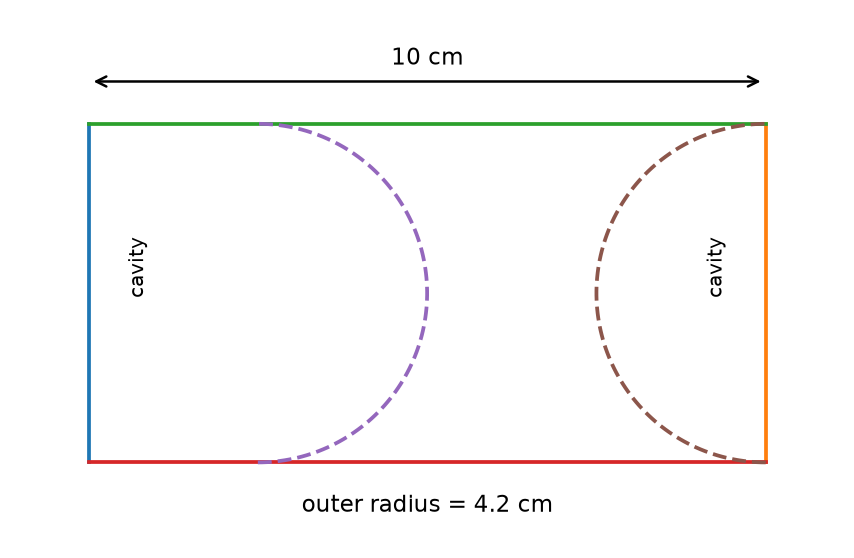
\includegraphics[width=0.84\linewidth]{../CBSE-2015-Class10-Updated-corrected_V3/figs/CylinderScooped.png}\caption{Two hemispherical cavities remove the volume of one sphere.}\label{fig:cylinder-scooped}\end{figure}
\solution The two hemispherical cavities together have the volume of one sphere. The remaining metal has volume
\begin{equation*}
V=\pi(4.2)^2(10)-\frac43\pi(4.2)^3=77.616\pi\,\mathrm{cm}^3\qquad\eqref{eq:cylinder-formula},\ \eqref{eq:sphere-formula},\ \eqref{eq:scooped-cylinder}.
\end{equation*}
The wire's thickness is its diameter, so its radius is $0.7$ cm. Equating the volumes gives
\begin{equation*}
\pi(0.7)^2L=77.616\pi\quad\Longrightarrow\quad L=\frac{77.616}{0.49}=158.4\,\mathrm{cm}.
\end{equation*}


The cylinder-and-cavities diagram is generated by this script:
\par\smallskip
\noindent\textbf{Code reference -}
\par\noindent\fbox{\parbox{\dimexpr\linewidth-2\fboxsep-2\fboxrule\relax}{\centering\texttt{../CBSE-2015-Class10-Updated-corrected_V3/codes/Q31.py}}}
\par\smallskip\end{enumerate}
